\documentclass[25pt, a0paper, portrait]{tikzposter}
\usetikzlibrary{fit,arrows,tikzmark,shadows,calc,automata}
\newcommand\NameBlock[1]{\node[fit=(blockbody)(blocktitle),inner sep=5pt] (#1) {};}
\usepackage[utf8]{inputenc}
\usepackage{subcaption}
\usepackage{adjustbox}
\usepackage{booktabs}

\usepackage[backend=bibtex]{biblatex}
\addbibresource{poster.bib}

\usepackage{authblk}
\makeatletter
% revert \maketitle to its old definition
% \def\maketitle{\AB@maketitle}
\renewcommand\maketitle{\AB@maketitle}

% put affiliations into one line
\renewcommand\AB@affilsepx{\quad\protect\Affilfont}
%
\makeatother
% set font for affiliations
\renewcommand\Affilfont{\Large}


\tikzposterlatexaffectionproofoff

% \usepackage{poster-style}
\usepackage{filecontents}
\usepackage{listings}


\title{FAT-Pointer based range TLB}
% \author{}
\date{\today}
% \institute{Heriot-Watt University UK \and Université de Toulouse France,
% and Carleton University Canada}

\author[1]{\Large Akilan Selvacoumar}
\author[1]{ Robert Stewart}
\author[1]{ Hans-Wolfgang Loidl}
\author[1]{ Ryad Soobhany}
\affil[1]{Heriot-Watt University, UK}

% \titlegraphic{
% 
\includegraphics[width=0.1\paperwidth]{hw-logo.png}
% }

\usepackage{blindtext}
\usepackage{comment}

% Default, Rays, Basic, Simple, Envelope, Wave, Board, Autumn, Desert
%
% good: Default, Basic, Simple
\usetheme{Basic}

% \renewcommand{\titleposright}{50mm}
% \titleposright=100mm
\definetitlestyle{sampletitle}{
  innersep=-10pt,
  titletotopverticalspace=-400mm,
  titletoblockverticalspace=10mm
}
{}

\usetitlestyle{sampletitle}
% \titleposleft=-300mm

% \usetitlestyle[titletotopverticalspace=-50mm,]{Basic}


% Britain, Australia, Sweden, Spain,Russia,Denmark,Germany
\usecolorstyle{Default}



\begin{document}
%   SICSA Postdoctoral and Early Career Researcher Exchanges.};

% removes space at top
\maketitle[titletotopverticalspace=-5mm]
% \maketitle

% \block{~}
% {
% \blindtext
% }

\begin{columns}
  \column{0.5}

  \block{Abstract}{

    % \begin{minipage}[t]{0.6\linewidth}

      \begin{tikzfigure}
        % \includegraphics[width=0.4\textwidth]{images/abstraction-poster.jpg}
      \end{tikzfigure}
      The CHERI architecture is designed to provide security guranetees, This has had performance implications such as more L1 TLB misses on
purecap mode rather than running an application as a 64 bit program. The following expirement proposes on adding range TLB which is
stored on the page table to store TLB translation entries of large memory objects (This would inturn lookup TLB entries in the range table
rather than looking up the L1 TLB entry). During this process the range ID would be added to the pointer which allows looking up the TLB
entries at an earlier stage during the pipeline. The FAT pointer structure of CHERI allows to encode custom bits of meta-data which in this
case can be used to store the ID of the range TLB entry.



    \vspace{0.5cm}
  }

  \block{Research Questions and Goals}{

    \hspace{0.5cm}

    \begin{minipage}[t]{0.8\linewidth}
      \textbf{\textit{Research Questions:}}
      \begin{itemize}
        \item (RQ1) Is there an optimization that explicitily uses FAT pointers to reduce the number of TLB misses to reduce the CPU STALL Time ?
        \item (RQ2) Can the number of L1 DTLB misses be minised by offloading translation lookups to the newly
        introduced range TLB ?
        % monolithic OS or containers in terms of wall-clock runtimes, CPU
        % profiling and memory profiling?
      % \item \textit{parallelising actors can increase throughput}
      \end{itemize}

    \end{minipage}%
    \hspace{0.2cm}

    \vspace{0.1cm}

    \begin{tikzfigure}
      % \includegraphics[width=0.4\textwidth]{images/parallel-layers-poster.png}
    \end{tikzfigure}

    \vspace{-0.5cm}
  }

  \block{Expirement Proposal}{

    \begin{minipage}[t]{0.4\linewidth}
      \vspace{-0.9cm}
      \begin{tikzfigure}{}
        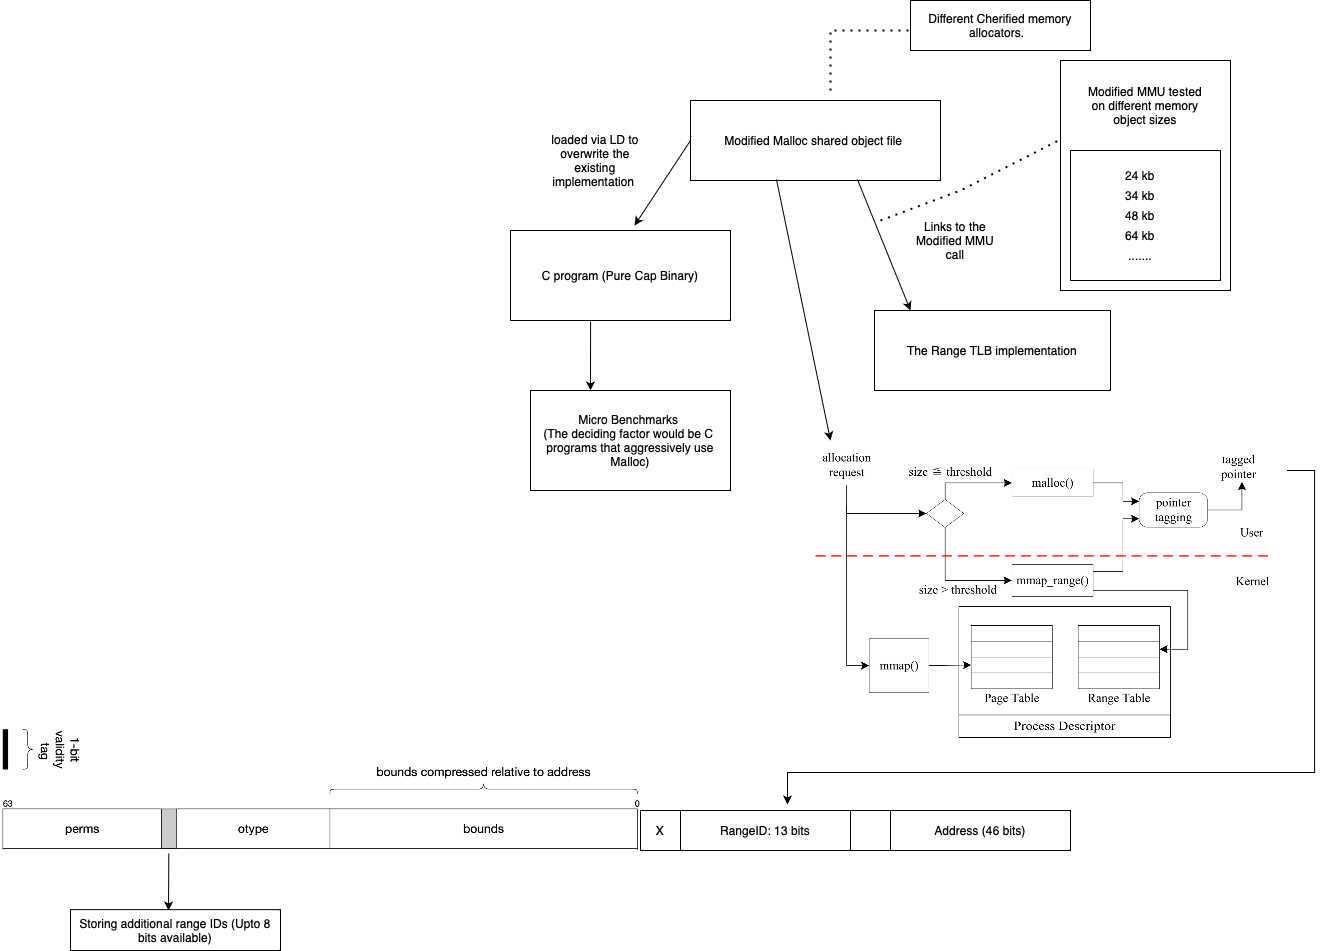
\includegraphics[width=2.53\textwidth]{Draft-expirment.png}
      \end{tikzfigure}
    \end{minipage}

    \vspace{0.6cm}

    % The following section describes the strategies used to measure distributed map-reduce applications on unikernels.
    % The metrics and scenarios measured would help towards the short-term goal of understanding the benefits of unikernels with
    % distributed map reduce.
    \hspace{0.5cm}
    \begin{minipage}[t]{0.8\linewidth}

      % \begin{itemize}
      % % \item \textbf{\textit{Benchmark application}}
      % %   \begin{itemize}
      % %   \item \textit{Mandelbrot}: The Mandelbrot Go implementation was used to
      % %   benchmark parallelised applications on Uni-kernels. The implementation uses
      % %   Go routines to spawn multiple threads. The parts parallelised of the Mandelbrot
      % %   implementation was the render part ,particularly the Mandelbrot iteration and
      % %   Linear interpolation.
      % %   \end{itemize}
      % % \item \textit{parallelising actors can increase throughput}
      % \end{itemize}

      % \begin{itemize}
      %   \item \textbf{\textit{Comparators}}
      %     \begin{itemize}
      %     \item \textit{Unikernel}
      %     \item \textit{Monolithic OS}
      %     \item \textit{Docker Container}
      %     \end{itemize}
      %   % \item \textit{parallelising actors can increase throughput}
      %   \end{itemize}

        % \begin{itemize}
        %   \item \textbf{\textit{Benchmark Metrics}}
        %     \begin{itemize}
        %     \item \textit{Boot-up time}
        %     \item \textit{Wall clock run times}
        %     \item \textit{Parallel Speed ups}
        %     \item \textit{Parallel efficiency}
        %     \end{itemize}
        %   % \item \textit{parallelising actors can increase throughput}
        %   \end{itemize}

    \end{minipage}%
    \hspace{0.2cm}

    \vspace{0.1cm}

    \begin{tikzfigure}
      % \includegraphics[width=0.4\textwidth]{images/parallel-layers-poster.png}
    \end{tikzfigure}

    \vspace{-0.5cm}
  }

  \NameBlock{transformation}
  \block{Exploiting CHERI pointers}{
    \hspace{0.4cm}
    % Bootup-times
    \begin{minipage}[t]{0.4\linewidth}
      \vspace{-0.9cm}
      \begin{tikzfigure}{}
        %  \includegraphics[width=2.47\textwidth]{Bootup-times.png}
      \end{tikzfigure}
    \end{minipage}



 }

    \NameBlock{transformation}
    \block{References}{
      \hspace{0.4cm}

    %  \begin{itemize}
    %    \item Building a parallel benchmark suite for Unikernels.
    %    \item Analysing the metrics provided by the Go compiler such as Heap usage, Number OS threads created by run time etc…
    %    \item Benchmarking other Unikernel implementation using the benchmark suite (1)
    %  \end{itemize}



   }

  \column{0.5}


  % \NameBlock{results}
  % \block{Experimental Setup (Mandelbrot program)}{
  %    \hspace{0.4cm}

  %   \begin{minipage}[t]{0.4\linewidth}
  %     \vspace{-0.9cm}
  %     \begin{tikzfigure}{}
  %       \includegraphics[width=2.54\textwidth]{expirement.png}
  %     \end{tikzfigure}
  %   \end{minipage}

  %   \vspace{0.4cm}

  %   \begin{itemize}
  %     \item \textit{Scenario 1\/}: Height of 1000 and 3000 iterations.
  %     \item \textit{Scenario 2\/}: Height of 2000 and 6000 iterations.
  %   \end{itemize}

  %   % \hspace{0.2cm}

  %   \begin{minipage}[t]{0.8\linewidth}

  %   \end{minipage}%

  %   \begin{tikzfigure}
  %     % \includegraphics[width=0.4\textwidth]{images/parallel-layers-poster.png}
  %   \end{tikzfigure}

  %   \vspace{-2.5cm}
  % }

%   \block{Results}{
%     \vspace{0.4cm}

%    \begin{minipage}[t]{0.4\linewidth}
%     %  \hspace{-0.9cm}
%      \textbf{\textit{Wall clock run times}}
%      \begin{tikzfigure}{}
%        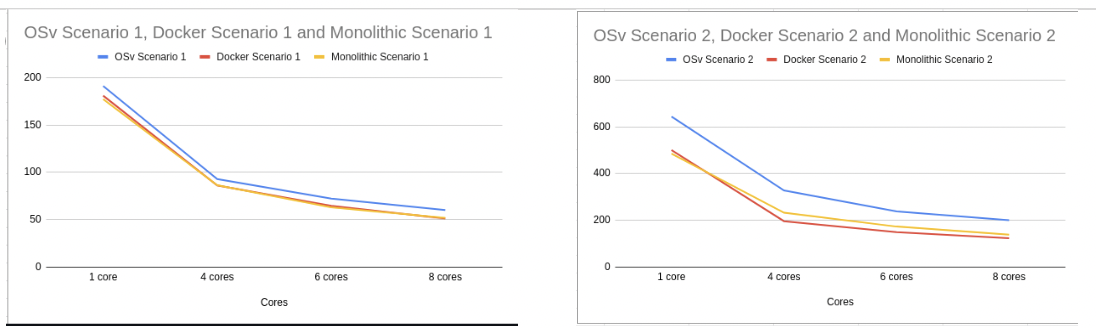
\includegraphics[width=2.54\textwidth]{WallClockRunTimes.png}
%      \end{tikzfigure}
%    \end{minipage}
%    \hspace{0.8cm}

%    \vspace{0.8cm}
%    \begin{minipage}[t]{0.4\linewidth}
%     % \vspace{-0.9cm}
%     \textbf{\textit{Parallel Speedups}}
%     \begin{tikzfigure}{}
%       \includegraphics[width=2.54\textwidth]{ParallelSpeedups.png}
%     \end{tikzfigure}
%   \end{minipage}

%   \vspace{0.8cm}
%   \begin{minipage}[t]{0.4\linewidth}
%     % \vspace{-0.9cm}
%     \textbf{\textit{Parallel Efficiency}}
%     \begin{tikzfigure}{}
%       \includegraphics[width=2.54\textwidth]{ParallelEffciency.png}
%     \end{tikzfigure}
%   \end{minipage}

%    % \hspace{0.2cm}

%    \begin{minipage}[t]{0.8\linewidth}

%    \end{minipage}%

%    \begin{tikzfigure}
%      % \includegraphics[width=0.4\textwidth]{images/parallel-layers-poster.png}
%    \end{tikzfigure}

%    \vspace{-2.5cm}
%  }

    % \NameBlock{model-checking}

  % \block{Conclusion}{
  %   \vspace{0.3cm}
  %   The empirical evidence gained from
  %   these measurements, running two different scenarios, will be used
  %   to answer the three research questions stated in the introduction
  %   of the paper. The empirical data from running the experiments on
  %   unikernels will provide a better understanding on how unikernels
  %   perform on a distributed memory environments.

  %   \vspace{1cm}

  %   \mbox{}\vspace{-\baselineskip}

  %   \printbibliography[heading=none]

  % }


\end{columns}

\begin{columns}
  \column{0.5}



  \column{0.5}

  \end{columns}

\end{document}
